\documentclass{report}

\usepackage[english]{babel}
\usepackage[utf8]{inputenc}
\usepackage{hyperref}

\usepackage{fancyhdr}
\usepackage {amsmath,amssymb} 
\usepackage{graphicx}
\usepackage{tikz-cd}
\usepackage{float}
\usepackage{amsthm}
\usepackage[all]{xy}
\usepackage[font={footnotesize}]{caption}

\usetikzlibrary{arrows}
\usetikzlibrary{matrix}


\newtheorem*{thm}{Theorem}
\newtheorem*{prop}{Proposition}
\newtheorem*{lemma}{Lemma}
\newtheorem*{coroll}{Corollary}     
\theoremstyle{definition}
\newtheorem*{defi}{Definition}
\newtheorem*{ex}{Example} 
\newtheorem*{exs}{Examples}
\theoremstyle{remark}
\newtheorem*{rk}{Remark}

 \newcommand{\Tt}{\ensuremath{ \{T(t)\}}}
\newcommand{\id}{\ensuremath{\text{I}}}
\newcommand{\la}{\ensuremath{_{\ast}}}
\newcommand{\upa}{\ensuremath{^{\ast}}}

\title{Complex Networks}
\author{{Marco Murtinu, Claudio Peroni}}

\begin{document}
	\maketitle
\section*{Introduction}	
The dataset we are going to analyze contains information about the email communications between 1005 people working in the same university. For each person we know to which department of the university they belong. There are 42 departments: we do not know the departments' names, they are just labeled from 0 to 41.

Since each node (person) can send as well as receive mails, the natural way to model this situation is a directed graph where each node respresents a person and each edge represents an email beetwen two people: particularly, for a node $n$, an inner-edge represents the receipt of an email, while an outer-edge means that he sent an email. Each node possesses the attribute \textit{department} which represents, of course, their department as an integer.

It is good practice to start any data analysis by cleaning the data: in this case we decided to remove all the self-loops in the graph. Indeed, they indicate the mails to one self, which are irrelevant to the analysis. The resulting graph, is visible in Figure \ref{fig:mail_graph}.

We also created an alternative, undirected version of the graph: we will see that this will be useful for some analysis and some interesting comparisons in the proceeding of this work. Clearly, we are aware that this two versions of the graph do have some differences, the most notable one being the numbers of edges and, consequently, the degree of nodes.
\bigskip

DIRECTED VERSION:

\begin{itemize}
\item Number of nodes: 1005
\item Number of edges: 24929
\item Average in degree: 24.8050
\item Average out degree: 24.8050
\end{itemize}


UNDIRECTED VERSION:

\begin{itemize}
	\item Number of nodes: 1005
	\item Number of edges: 16064
	\item Average degree: 31.9682
\end{itemize}

\begin{figure} [H]
	\centering
	\centerline{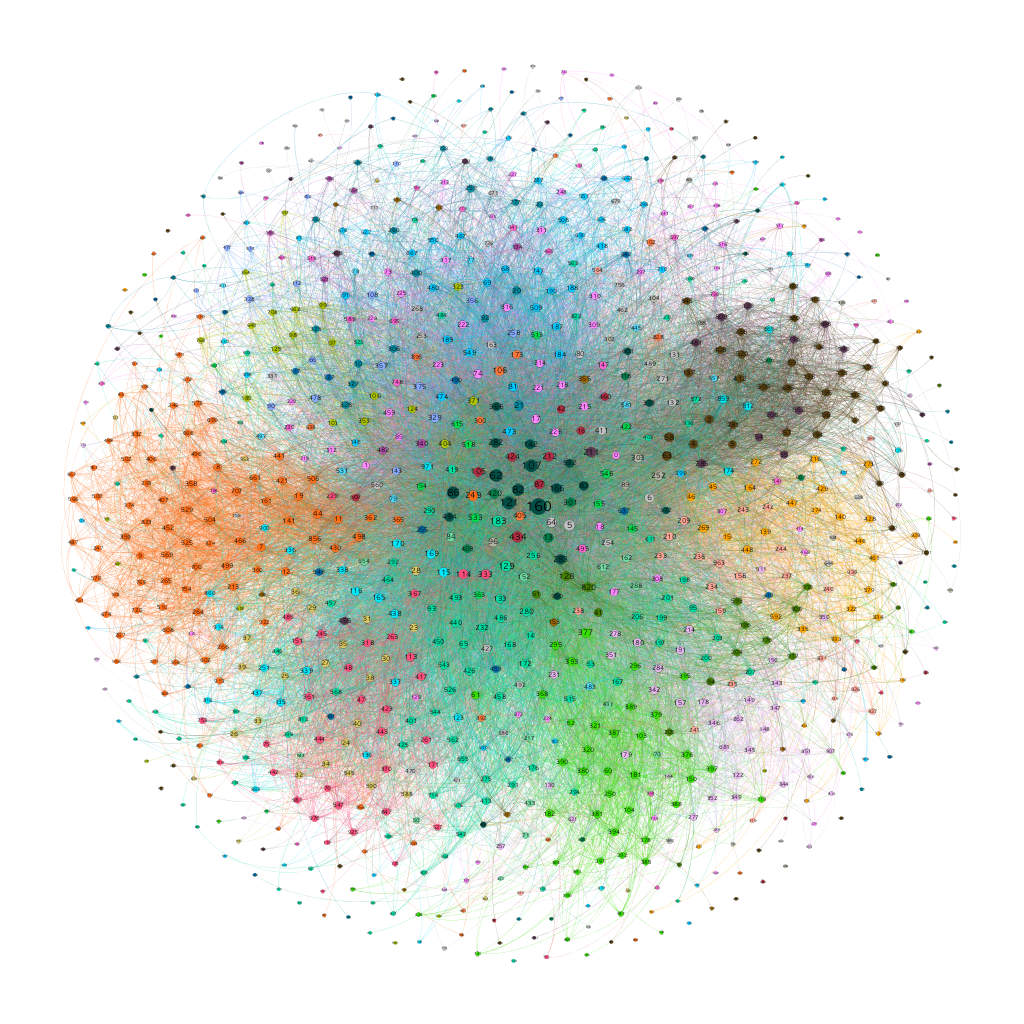
\includegraphics[width = 24cm, height = 18cm, keepaspectratio]{eMail_graph.png}}
	\caption{Emails graph: the size of nodes is proportional to their degree, the colors represent the modularity class assigned by Gephi. The colors of the edges denote the modularity class of the source.} \label{fig:mail_graph}
\end{figure}

We created another related graph, visible in Figure \ref{fig:dep_graph}, representing only the departments: this is an undirected weighted graph having the departments as nodes, where the edge between two departments has a weight proportional to the number of communications between their elements. We will see that this graph will be useful to draw further conclusions, looking at the data with an aggregate perspective. Here is a summary of this graph:

\begin{itemize}
	\item Number of nodes: 42
	\item Number of edges: 679
	\item Average degree: 32.3333
\end{itemize}
\begin{figure} [H]
	\centering
	\centerline{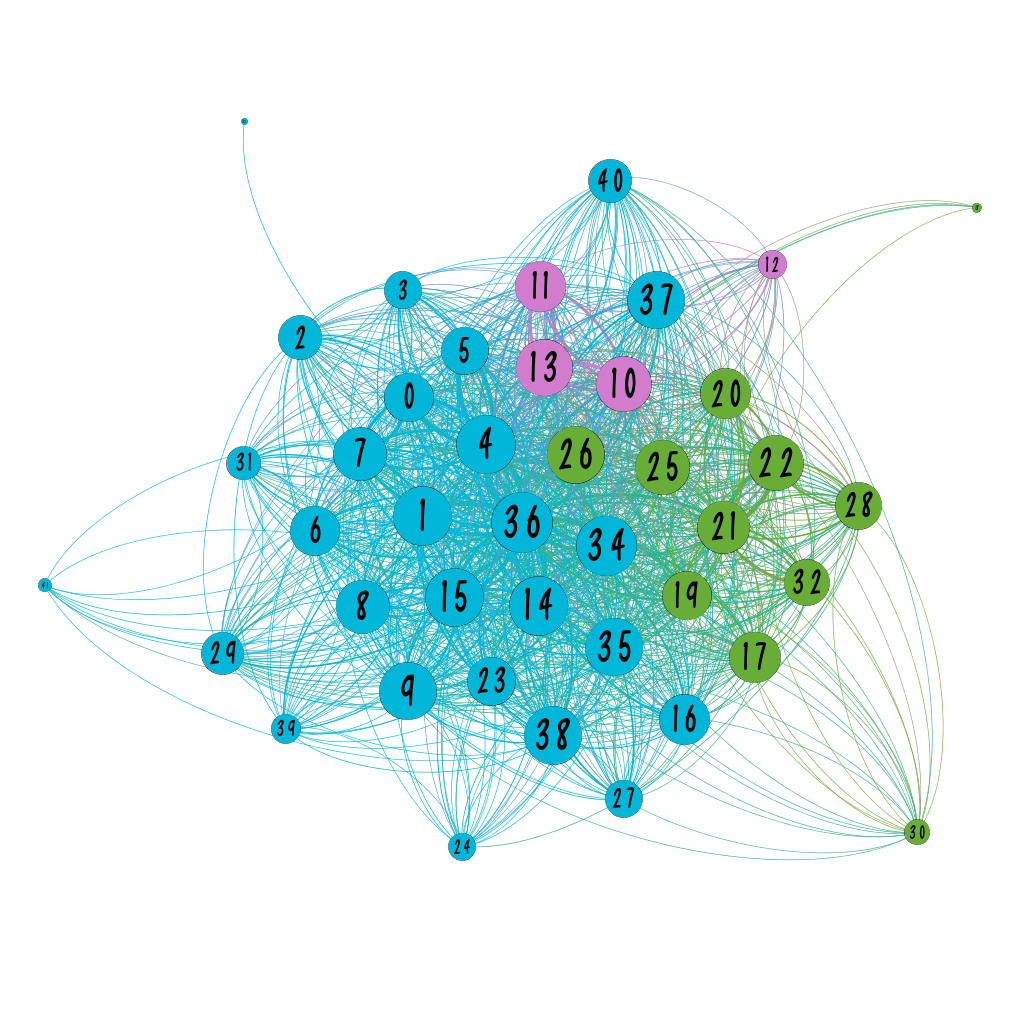
\includegraphics[width = 12cm, height = 14cm, keepaspectratio]{Departments_graph.png}}
	\caption{Departments graph: the size of nodes is proportional to their weighted degree, the colors represent the modularity class assigned by Gephi.} \label{fig:dep_graph}
\end{figure}
\section*{Connected components and Giant component}

We begin our study by analyzing the structure of the network.

First, we search for the weakly and strongly connected components in both the directed and the undirected mail graphs.
\begin{itemize}
	\item Number of connected components (undirected version): 20
	\item Number of weakly connected components: 20
	\item Number of strongly connected components: 203
\end{itemize}


Clearly, the number of connected components of the undirected graph is the same as the number of weakly connected components of the directed graph, as expected by definition.

It comes as no surprise that the strongly connected components are much more than the weakly connected components, since the latter is a easier requirements to meet: recall that a directed graph is said to be \textbf{strongly connected} if any vertex is reacheable from every other vertex, whereas a directed graph is \textbf{weakly connected} if, by substituting all its edges with undirected edges, we obtain a connected graph.

Speaking about connected components, it is of considerable interest to understand whether there exists a \textbf{giant component}, i.e., a connected component that contains a significant fraction of all nodes. Let us start from the undirected version of the graph, which has only 20 connected components.
\bigskip


COMPONENT 0:
\begin{itemize}
\item Number of nodes: 986
\item Number of edges: 16064
\item Relative Order (proportion of nodes): 0.9811
\item Relative Size (proportion of edges): 1.0\\
\end{itemize}

COMPONENT 1:
\begin{itemize}
\item Number of nodes: 1
\item Number of edges: 0
\item Relative Order (proportion of nodes): 0.0010
\item Relative Size (proportion of edges): 0.0\\
\end{itemize}


COMPONENT 2:
\begin{itemize}
\item Number of nodes: 1
\item Number of edges: 0
\item Relative Order (proportion of nodes): 0.0010
\item Relative Size (proportion of edges): 0.0\\
\end{itemize}

$\vdots$

COMPONENT 19:
\begin{itemize}
\item Number of nodes: 1
\item Number of edges: 0
\item Relative Order (proportion of nodes): 0.0010
\item Relative Size (proportion of edges): 0.0\\
\end{itemize}

It is easy to see that the first component represents a giant component: indeed it contains more than $98\%$ of all the nodes and all the edges of the graph, whereas the other 19 components are all composed by a single node (they are what we may call detached leaves).

Let us now try to find a giant component also in the directed graph.
\bigskip 

COMPONENT 0:
\begin{itemize}
	\item Number of nodes: 1
	\item Number of edges: 0
	\item Relative Order (proportion of nodes): 0.0010
	\item Relative Size (proportion of edges): 0.0\\
\end{itemize}

COMPONENT 1:
\begin{itemize}
	\item Number of nodes: 1
	\item Number of edges: 0
	\item Relative Order (proportion of nodes): 0.0010
	\item Relative Size (proportion of edges): 0.0\\
\end{itemize}

$\vdots$

COMPONENT 162:
\begin{itemize}
	\item Number of nodes: 803
	\item Number of edges: 24138
	\item Relative Order (proportion of nodes): 0.7990
	\item Relative Size (proportion of edges): 0.9683\\
\end{itemize}

$\vdots$

COMPONENT 202:
\begin{itemize}
	\item Number of nodes: 1
	\item Number of edges: 0
	\item Relative Order (proportion of nodes): 0.0010
	\item Relative Size (proportion of edges): 0.0\\
\end{itemize}

Even in this case we easily recognize the giant component to be the component 162: it contains around $80\%$ of the nodes and more than the $96\%$ of all the edges of the graph. The other 201 components are composed just by a single node.

Eventually, we calculated also the number of connected components in the departments network: as expected, there is only one such component.
\newpage
\section*{Degree}

Let us now study the distribution of the degree among nodes.


\begin{figure} [H]
	\centering
	\centerline{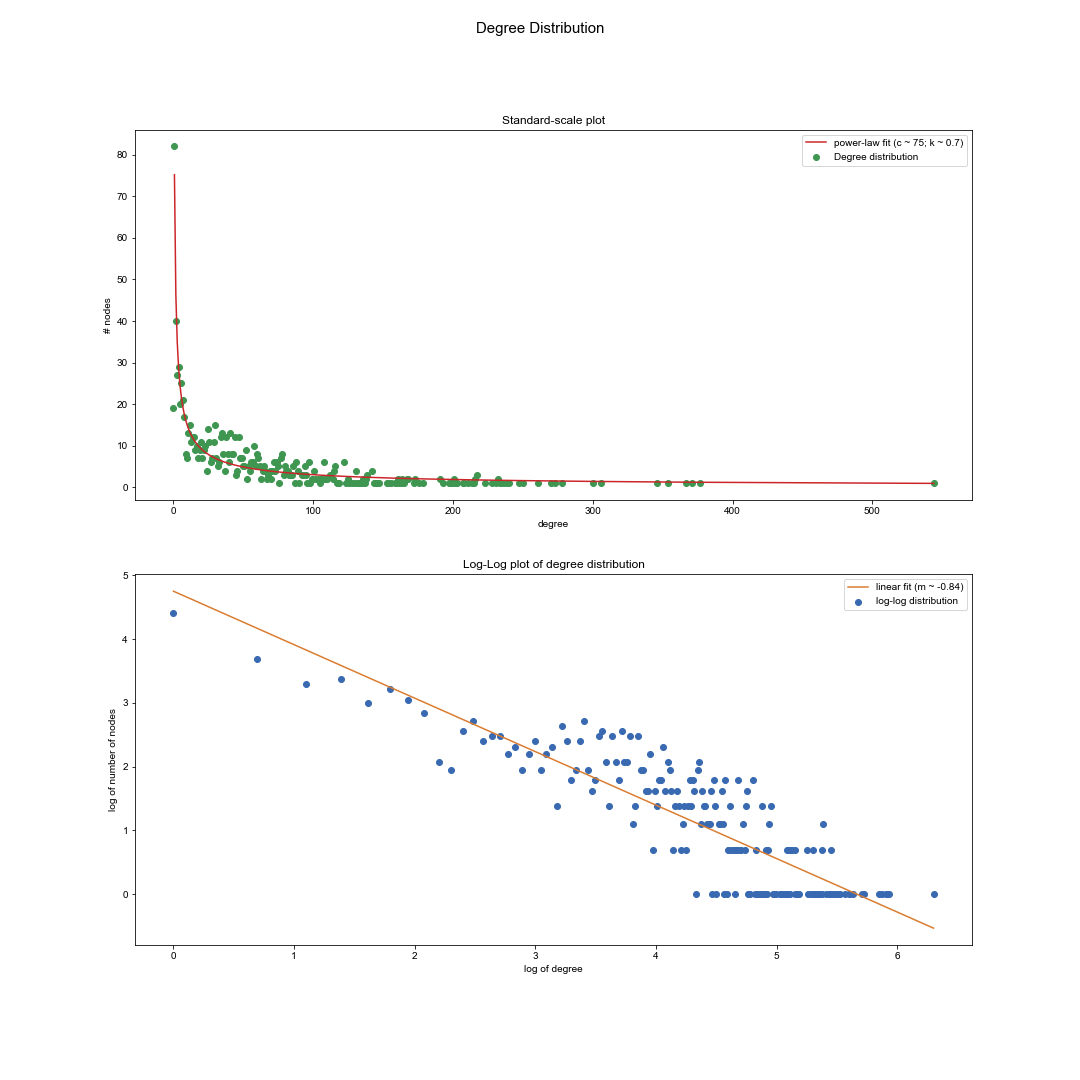
\includegraphics[width = 18cm, height = 14cm, keepaspectratio]{degree_distribution_fit.png}}
	\label{Degree}
	\caption{The first graph represents the degree distribution: its shape resembles a power law, therefore, in order to confirm it, we plot it again after a log transformation. The red lines represent the theoretical power-law that best fits the data. In both cases we can say that the data roughly follow a power-law, at least to some extent.}
\end{figure}

The first plot shows the degree distribution of the nodes: its shape resembles, to some extent, a power-law, which may be reasonable since the degree of a node can be intended as a kind of popularity measure of the node itself. However the first plot is not enough to fully confirm such hypothesis, therefore we apply a logarithmic transformation. Indeed, if $f(k)$, the function representing the frequency of the degree $k$ among nodes, follows a power-law, then
\begin{equation*}
f(k)  = \frac{a}{k^c}
\end{equation*}
where $a$ is a constant of proportionality. Our aim is to find $c$. Hence we apply a log transformation, so to have
\begin{equation*}
\log(f(k)) = \log(a) -c \log(k)
\end{equation*}
In this setting, $a$ is the intercept with the $y$ axis and $c$ is the slope of the line. In the second plot we can roughly see a line with slope between 1 and $5/6$, which supports the power-law hypothesis to some extent.

We also compute the average degree, the maximum degree and the standard deviation of this distribution
\begin{itemize}
	\item Average degree : 49.6099
	\item Standard deviation: 59.7496
	\item Maximum degree: 544\footnote{Note that this degree belongs to node 160, which will appear again and again in this analysis, being the most central node in the graph with a degree way above that of the others.}
\end{itemize}
It may be of interest to study the degree's distribution also in the department graph. Note that, differently from what we have found in the emails graph, the plots below strongly deviate from the theoretical behavior of a power-law.
\begin{figure} [H]
	\centering
	\centerline{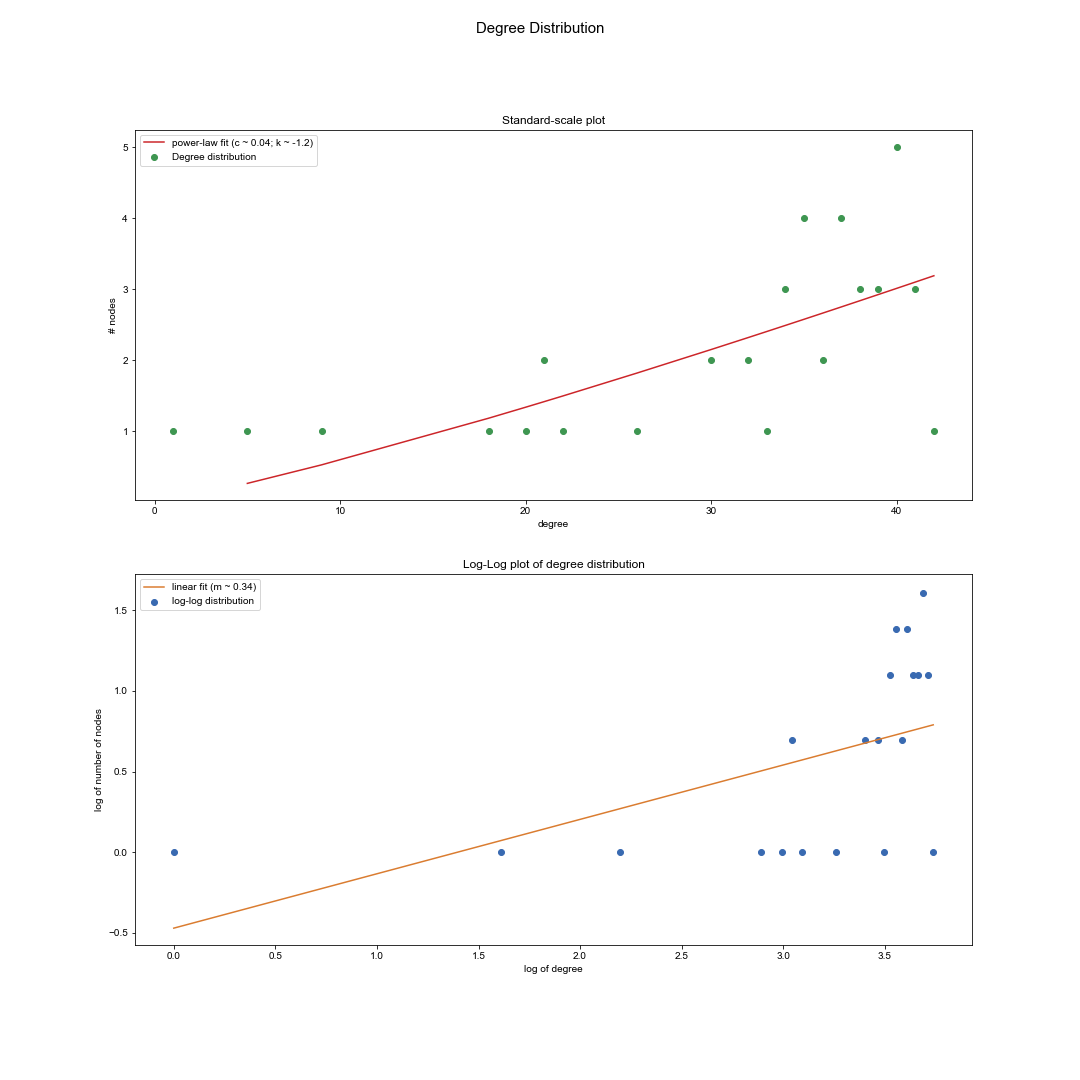
\includegraphics[width = 18cm, height = 14cm, keepaspectratio]{DEP_degree_distribution.png}}	\caption{Degree distribution in the departments graph: in the first plot we have the degrees on the $x$-axis and their frequences on the $y$-axis. In the second one we applied a log transformation to better evaluate the presence of a power law distribution, which is clearly not present.}
\end{figure}
\newpage
\section*{Distances}
We now compute the distribution of distances: it is important to stress that in this analysis we are bound to consider only the \textit{giant strongly connected component} for the directed graph and the \textit{giant connected component} for the undirected graph, otherwise we would obtain infinite values. Let us first study the directed graph.
\begin{figure} [H]
	\centering
	\centerline{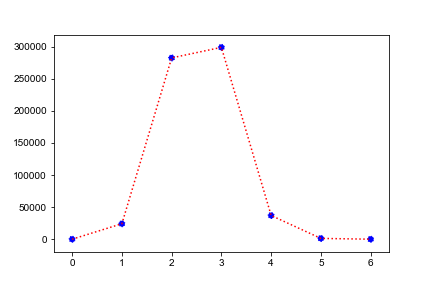
\includegraphics[width = 13cm, height = 12cm, keepaspectratio]{distance_distribution.png}}
	\label{Dist}
	\caption{Distance distribution in the directed graph.}
\end{figure}
 We then compute some statistics of such distribution\footnote{Note that for this analysis we decided to exclude the null distances, \textit{i.e.} all the distances between any node and itself, which will always be the same number as the number of nodes.}:
 \begin{itemize}
 	\item Average distance in the strongly connected component: 2.5443
 	\item Standard deviation of distance in the strongly connected component: 0.6757
 \end{itemize}
Let us now do the same for the undirected graph.
\begin{figure} [H]
	\centering
	\centerline{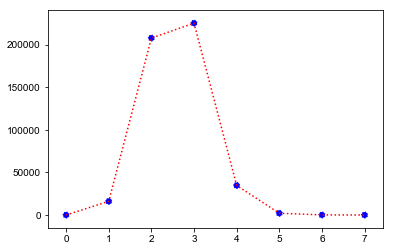
\includegraphics[width = 13cm, height = 12cm, keepaspectratio]{distance_distribution_und.png}}
	\label{Dist_und}
	\caption{Distance distribution in the undirected graph.}
\end{figure}
Once more, we compute the average and standard deviation of the distribution:
 \begin{itemize}
	\item Average distance in the connected component: 2.5843
	\item Standard deviation of distance in the connected component: 0.6970
\end{itemize}
To conclude our discussion about distances in the emails network, we compute the \textit{eccentricities} in the strongly giant component as well as in the giant component. In both cases, we report the diameter and the radius of the networks (which are the \textit{max} and \textit{min} eccentricities respectively).
\begin{itemize}
	\item Radius of the giant strongly connected component: 3
	\item Radius of the giant connected component: 4
	\item Diameter of the giant strongly connected component: 6
	\item Diameter of the giant connected component: 7
\end{itemize}
We see that the giant strongly connected component (with $\sim80\%$ of the nodes of the whole graph) effectively has a smaller radius and diameter than the giant connected component of the undirected graph (which has $\sim98\%$ of the nodes).

Once more, we conclude the analysis by studying the distance distribution also on the departments graph.
\begin{figure} [H]
	\centering
	\centerline{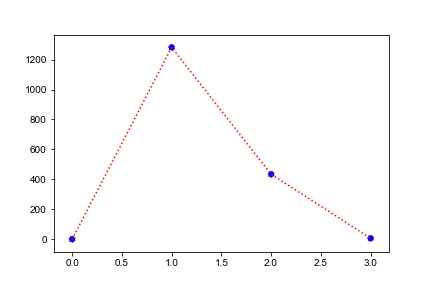
\includegraphics[width = 13cm, height = 12cm, keepaspectratio]{DEP_distance_distribution.png}}
	\label{Dist_dep}
	\caption{Distance distribution in the departments graph.}
\end{figure}
It is apparent how different the distribution of the distances in the \textit{mail network} and the one in the \textit{department network} are. This comes to no surprise, considering that for two departments to be neighbors it is sufficient that any two people inside them exchanged a single mail.
\section*{Centrality}
Understand which groups or single nodes are central for a network is not immediate: indeed there are several different measures of centrality, each focusing on a slightly different aspect and proposing and slightly different notion of centrality. However we will see that in our graph all these measures will agree in identifying the central group and the central node.

The first measure we compute is probably the simplest and most intuitive one, the \textbf{degree centrality}, which measures the centrality of a node by its degree, i.e., by the number of nodes connected to it. Unsurprisingly, coherently with that we obtained when we studied the degree distribution, we see that node number 160 is the most central node. Moreover, node 160 as well as all the other most central nodes, belongs to department 36, which is identified as the most central department.

A second measure of centrality is the \textbf{eigenvector centrality}: the idea underneath this measure is that a high eigenvector score means that a node is connected to many nodes who themselves have high scores. Despite using a different measure, we still find that node 160, belonging to department 36, is the one with highest eigenvector centrality.

Another possible measure is the \textbf{closeness centrality}, calculated as the sum of the lengths of the shortest paths between the node and all other nodes in the graph. For a node $n$ 
\begin{equation*}
C(n) = \sum_{m \neq n}\frac{1}{d(n,m)}
\end{equation*}
where $m$ is another node in the graph, is its closeness centrality.
Thus the more central a node is, the closer it is to all other nodes. Once more, the node 160 is the one with the highest centrality measure.

Eventually, we compute the \textbf{betweeness centrality}, defined as the number of shortest paths that pass through a node, i.e., 
\begin{equation*}
b(n) = \sum_{m \neq n\neq l} \frac{\sigma_{m,l}(n)}{\sigma_{m,l}}
\end{equation*}
where $\sigma _{m,l}$ is the total number of shortest paths from node $m$ to node $l$ and  $\sigma_{m,l}(n)$ is the number of those paths that pass through $n$. Also in this case, node 160 receives the highest score.

However, the situation becomes less clear when analyzing the centrality of the departments network: we are going to see that the centrality measures on this graph will support our previous conclusions only to some extent.

We have a first confirm of the centrality of the department 36, that we discovered in the emails network, by using the degree centrality: this department scores a value slightly higher than departments 1 and 15. The situation becomes less clear when computing the betwness centrality: in this case the department 4 gets a value significantly higher (0.0551) than the value of department 36 (0.0223).
\section*{Clustering coefficient}
First, we compute the average clustering coefficient for the whole graph. Note that in order to do this we need to use the undirected version.
\begin{itemize}
	\item Average clustering for undirected graph: 0.3994
\end{itemize}


We are also interested in checking the clustering coefficient of the most central node, 160, which is 0.0935.  


Note that the fact that the clustering coefficient of the most central node is very low makes sense: since it is connected to huge number of nodes, it would be strange if a lot of them were connected to each other; indeed, they can be far away from each other.

Let us now exploit the fact that we are aware of a natural partition of the nodes in the graph: departments. It may be interesting to see whether such natural groups form strongly clustered regions. Recalling that the average clustering coefficient of the network is around 0.4, we see that most departments, with the expection of those composed by just one node, which of course score 0, and those composed by just 2 nodes with a link between them, which clearly score 1, have a clustering coefficient significantly above the average.\\
\section*{Density}
Another measure of the thickness of the graph is its \textbf{density}, defined as the ratio between the number of edges between all the nodes and the number of all the possible edges between such nodes. We computed it for both the emails and the departments networks.
\begin{itemize}
	\item Density of email network: 0.0247
	\item Density of department network: 0.7886
\end{itemize}
As we might expect, the departments network is much more dense then the emails graph.
\section*{Homophily}
We would like to understand whether our network exhibits some sort of homophily. However, this analysis is difficult in our situation, becausee we do not know anything about the single node: the only information that we have about a person is his or her department, we do not know anything about his age, gender, nationality or other personal features with respect to analyze the homophily. Therefore, we are bound to try to compute the homophily with respect to the only information we have, the department. Note that this a "formal" homophily: we will basically understand whether people in the same department communicate more often with people within their department than with people of other departments.

To analyze homophily we consider a network in which the attribute "department" is randomly assigned to each node with probability proportional to the proportion of nodes belonging to that department in the original network. Therefore, denoting by $p_i$ the probability that a node belongs to department $i$, and considering two random nodes linked by an edge, the probability that they belong to the same department is
\begin{equation*}
\sum_{i=0}^{41} p_i^2
\end{equation*}
Hence the probability that they belong to different departments is
\begin{equation*}
1-\sum_{i=0}^{41} p_i^2 = 0.9524
\end{equation*}
Instead, considering our network and counting the proportion of edges between nodes belonging to different departments, we obtain 0.6643. This shows that in our graph there are significantly less edges that connect nodes from different departments than in a random graph with the same proportion of nodes in each department. Hence we can say that our network displays homophily.
\section*{Assortativity}
The \textbf{assortativity} represents the preference of a network's nodes to attach  to others that are similar in some way. We operationalize this idea by measuring assortativity, as it is common practice, with respect to nodes' degree.

The plot below clearly shows that there is no evidence for assortativity: indeed, in such a case, we would expect an increasing trend of the curve. By the same token, in case of dissortativity, we would expect a decreasing trend in the curve. In this case, we cannot see any of these behaviors, hence we must conclude that our network is neutral.
\begin{figure} [H]
	\centering
	\centerline{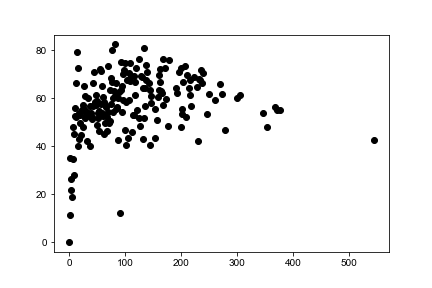
\includegraphics[width = 13cm, height = 12cm, keepaspectratio]{assortativity.png}}
	\label{Ass}
	\caption{Assortativity in the emails graph: there is no clear evidence neither for assortativity nor for dissortativity. We may conclude that the network is neutral.}
\end{figure}
As we have done for all the other analysis, let us see whether we can find assortativity in the departments graph. We can see that, differently from the emails network, the graph shows some dissortativity, having a degree assortativity coefficient of -0.1786. This suggests that departments with high degree are slightly incline to attach to departments with lower degree.
 \begin{figure} [H]
 	\centering
 	\centerline{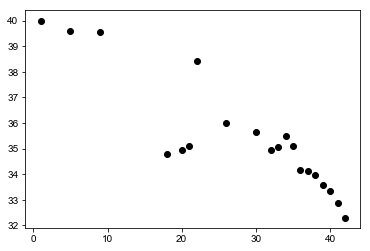
\includegraphics[width = 13cm, height = 12cm, keepaspectratio]{assortativity_dep.png}}
 	\label{Ass_dep}
 	\caption{Assortativity in the departments graph: the plot shows a certain degree of disassortativity.}
 \end{figure}
\end{document}